%----------------------------------------------------------------
%
%  File    :  thesis.tex
%
%  Authors :  Keith Andrews, IICM, TU Graz, Austria
%             Manuel Koschuch, FH Campus Wien, Austria
% 
%  Created :  22 Feb 96
% 
%  Changed :  24 March 2009
% 
%----------------------------------------------------------------

% Please send any questions, comments, remarks or complaints to
% manuel.koschuch@fh-campuswien.ac.at


% --- General Setup ---------------------------------------------

\documentclass[12pt,a4paper,oneside]{book}

%\usepackage{times}

%\renewcommand{\rmdefault}{phv} % Arial
%\renewcommand{\sfdefault}{phv} % Arial

\usepackage{listings}	%% added to avoid the \lstlistoflistings error

\usepackage[utf8]{inputenc}   % so can use Umlaut chars  ä, ü
\usepackage[ngerman]{babel}
\usepackage[T1]{fontenc}

\usepackage[bf,sf]{subfigure}
\renewcommand{\subfigtopskip}{0mm}
\renewcommand{\subfigcapmargin}{0mm}

\usepackage{url}
\usepackage{latexsym}
\usepackage{ifpdf} % detect outputstyle
\usepackage{geometry} % define pagesize in more detail
\usepackage{fancyhdr} % nicer headers and footers
\usepackage{colortbl} %define colored backgrounds for tables
\usepackage{multicol}

\ifpdf
  \usepackage[pdftex]{graphicx}
  \DeclareGraphicsExtensions{.pdf,.jpg,.png}
  \pdfcompresslevel=9
  \pdfpageheight=297mm
  \pdfpagewidth=210mm
  \usepackage[         % hyperref should be last package loaded
    pdftex,
    bookmarks,
    bookmarksnumbered,
    linktocpage,
    pagebackref,
    pdfview={Fit},
    pdfstartview={Fit},
    pdfpagemode=UseOutlines,                 % open bookmarks in Acrobat
  ]{hyperref}
  \usepackage{bookmark}
\else                      % latex
  \usepackage{graphicx}
  \DeclareGraphicsExtensions{.ps}
\fi

\geometry{a4paper,left=30mm,right=25mm, top=30mm, bottom=30mm}

\setlength{\parskip}{3pt plus 1pt minus 0pt}       % vert. space before a paragraph

\setcounter{tocdepth}{1}        % lowest section level entered in ToC
\setcounter{secnumdepth}{2}     % lowest section level still numbered
% --- Start of Document ----------------------------------------

\begin{document}

\frontmatter
\normalsize
\pagestyle{empty}            % for title pages

%----------------------------------------------------------------
%
%  File    :  title.tex
%
%  Authors :  Keith Andrews, IICM, TU Graz, Austria
%             Manuel Koschuch, FH Campus Wien, Austria
% 
%  Created :  22 Feb 96
% 
%  Changed :  22 February 2011
% 
%----------------------------------------------------------------


% --- Main Title Page ------------------------------------------------

% A4 paper =  w=21cm, h=29.7cm

%\setlength{\textheight}{26.83cm}
%\setlength{\textwidth}{17cm}
%
%\setlength{\oddsidemargin}{-0.04cm}
%\setlength{\topmargin}{-2.5cm}

%\pagestyle{fancyplain}
%\fancyhead{}
%\renewcommand{\headrulewidth}{0.0pt}
%\fancyhead[L]{\includegraphics[height=25mm]{images/logo.png}}
%\fancyfoot[C]{\fancyplain}

\vspace*{-2.5cm}

\begin{center}

\vspace{1.3cm}

\hspace*{-1.0cm} {\Large \textbf{iOS Jailbreak\\}}

\hspace*{-1.0cm} und die Auswirkungen auf die Sicherheit und Vertrauenswürdigkeit des Systems \\

\vspace{2.2cm}

\hspace*{-1.0cm} \textbf{Diplomarbeit\\}

\vspace{0.65cm}

\hspace*{-1.0cm} Zur Erlangung des akademischen Grades \\

\vspace{0.65cm}

\hspace*{-1.0cm} \textbf{Master of Science in Engineering (MSc)\\}

\vspace{0.65cm}

\hspace*{-1.0cm} der Fachhochschule Campus Wien \\
\hspace*{-1.0cm} Masterstudiengang IT-Security \\

\vspace{5cm}

\hspace*{-1.0cm} \textbf{Vorgelegt von:} \\
\hspace*{-1.0cm} Michael Fuska, BSc \\

\vspace{0.65cm}

\hspace*{-1.0cm} \textbf{Personenkennzeichen}\\
\hspace*{-1.0cm} c1410537032 \\

\vspace{2.1cm}

\hspace*{-1.0cm} \textbf{Erstbegutachter/in:} \\
\hspace*{-1.0cm} Katharina Krombholz, MSc \\

\vspace{0.5cm}

\hspace*{-1.0cm} \textbf{Zweitbegutachter/in:} \\
\hspace*{-1.0cm} Dr. Martin Mulazzani, \\


\vspace{1.4cm}

\hspace*{-1.0cm} \textbf{Eingereicht am:} \\
\hspace*{-1.0cm} 07.08.2016 \\

\end{center}

\newpage

\pagestyle{empty}

\vspace*{16.5cm}  %% change from 17cm to 16.5cm to avoid an empty page

\hspace*{-0.7cm} \underline{Erklärung:}\\\\
Ich erkläre, dass die vorliegende Diplomarbeit von mir selbst verfasst wurde und ich keine anderen als die angeführten Behelfe verwendet bzw. mich auch sonst keiner unerlaubter Hilfe bedient habe.\\
Ich versichere, dass ich dieses Diplomarbeitsthema bisher weder im In- noch im Ausland (einer Beurteilerin/einem Beurteiler zur Begutachtung) in irgendeiner Form als Prüfungsarbeit vorgelegt habe.\\
Weiters versichere ich, dass die von mir eingereichten Exemplare (ausgedruckt und elektronisch) identisch sind.\\\\
Datum: \hspace{6cm} Unterschrift:\\






              % Title Page

\pagestyle{fancy} 
\fancyhf{}
	
\setlength{\headheight}{15pt}
\renewcommand{\headrulewidth}{0.0pt}

\fancyfoot[R]{\thepage}      
\pagenumbering{roman}        % for preliminary pages

%----------------------------------------------------------------
%
%  File    :  acknowl.tex
%
%  Authors :  Keith Andrews, IICM, TU Graz, Austria
%             Manuel Koschuch, FH Campus Wien, Austria
% 
%  Created :  22 Feb 96
% 
%  Changed :  30 Oct 2008
% 
%----------------------------------------------------------------

\begin{center}
{\Large\bfseries Danksagung}
\end{center}

(Falls gewünscht.)          % Acknowledgements
%----------------------------------------------------------------
%
%  File    :  abstracts.tex
%
%  Authors :  Keith Andrews, IICM, TU Graz, Austria
%             Manuel Koschuch, FH Campus Wien, Austria
% 
%  Created :  22 Feb 96
% 
%  Changed :  30 Oct 2008
% 
%----------------------------------------------------------------


% --- German and English Abstracts ------------------------------------------------

% --- German Abstract ----------------------------------------------------
\cleardoublepage

\begin{center}
{\Large\bfseries Kurzfassung}
\end{center}


(Z.B. ``Diese Arbeit beschäftigt sich mit...'')


% --- English Abstract ----------------------------------------------------

\cleardoublepage

%\selectlanguage{english}

\begin{center}
{\Large\bfseries Abstract}
\end{center}

(E.g. ``This thesis deals with...'')

%\selectlanguage{austrian}
        % Englisch and German abstracts
%----------------------------------------------------------------
%
%  File    :  glossary.tex
%
%  Author  :  Manuel Koschuch, FH Campus Wien, Austria
% 
%  Created :  30 Oct 2008
% 
%  Changed :  30 Oct 2008
% 
%----------------------------------------------------------------

\begin{center}
{\Large\bfseries Abkürzungsverzeichnis}
\end{center}

\begin{table*}[htbp]
		 \begin{tabular}{p{3cm}p{12cm}} 
		    \textbf{AES} & Advanced Encryption Standard \\
            \textbf{AES-CBC} & Advanced Encryption Standard Cipher Block Chaining \\
            \textbf{AES-XTS} & Advanced Encryption Standard XEX-based tweaked-codebook mode with ciphertext stealing \\ 
		     \textbf{ASLR} & Address space layout randomization \\
		     \textbf{AFC} & Apple File Conduit\\
		     
		     \textbf{BYOD} & Bring Your Own Device\\
		     
		     \textbf{CTR-DRBG} & Counter mode Deterministic Random Byte Generator \\
		     
		     \textbf{DFU Mode} & Device Firmware Upgrade Mode\\
		     \textbf{DDI} & Development Disk Image \\
		     \textbf{DMA} & Direct Memory Access\\
		     \textbf{DTLS} & Datagram Transport Layer Security \\
		     
		     \textbf{GID} & Group ID \\
		     \textbf{GQM} & Goal Question Metric Methode \\
		     
		     \textbf{HTML} & Hypertext Markup Language \\
		     
		     \textbf{IPsec} & Internet Protocol Security \\
		     \textbf{iOS} & iPhone Betriebssystem\\
		     
		     
		     \textbf{MDM} & Mobile Device Management \\
		     
		     \textbf{NFC} & Near Field Communication \\
             
             \textbf{JIT} & Just In Time \\		     
		     
		     \textbf{SGML} & Standard Generalized Markup Language \\
 		     
 		     \textbf{TLS} & Transport Layer Security \\
 		     
 		     \textbf{UID} & Unique ID \\
 		     
 		     \textbf{RNG} & Random Number Generator\\
 		     \textbf{RPC} & Remote Procedure Call \\
 		     
 		     \textbf{UDID} & Unique Device Identifiers\\
 		     \textbf{UUID} &  Universally Unique IDentifier \\
 		 	 
 		 	 \textbf{VPN} & Virtual Private Network \\
		\end{tabular}
\end{table*}         % Glossary
%----------------------------------------------------------------
%
%  File    :  keywords.tex
%
%  Author  :  Manuel Koschuch, FH Campus Wien, Austria
% 
%  Created :  30 Oct 2008
% 
%  Changed :  30 Oct 2008
% 
%----------------------------------------------------------------

\begin{center}
{\Large\bfseries Schlüsselbegriffe}
\end{center}

\noindent
\textbf{iOS Sicherheitsmechanismen } \\
\textbf{Jailbreak } \\
       % Keywords
%----------------------------------------------------------------
%
%  File    :  toc.tex
%
%
%  Authors :  Keith Andrews, IICM, TU Graz, Austria
%             Manuel Koschuch, FH Campus Wien, Austria
% 
%  Created :  22 Feb 96
% 
%  Changed :  30 Oct 2008
% 
%----------------------------------------------------------------

{
\setlength{\parskip}{3pt plus 3pt minus 3pt}     % compact table of contents

\tableofcontents
}
                 % Table of Contents

\mainmatter

\cleardoublepage
\renewcommand{\headrulewidth}{0.4pt}

\pagestyle{fancy}            % for main pages
\fancyhf{}
\fancyhead[RO]{\slshape \nouppercase{\leftmark}}
\fancyfoot[R]{\thepage}     
\pagenumbering{arabic}      % for main pages

%--- Include your chapters here ----------

%----------------------------------------------------------------
%
%  File    :  chapter1.tex
%
%  Authors : Michael Fuska, FH Campus Wien, Austria% 
%  Created : 13 Feb 2016
%
%  Changed :  
% 
%----------------------------------------------------------------


\chapter{Einleitung}
\label{ch:intro}


\section{Einführung}
\label{sec:Einführung}

Das Smartphone ist ein ständiger Begleiter des Menschen geworden. Es nimmt von Tag zu Tag mehr Einfluss auf unser Leben. Neben dem privaten Gebrauch ist es auch im beruflichen Alltag nicht mehr wegzudenken. Sensible Informationen und Daten werden auf dem Smartphone verarbeitet und/oder gespeichert. Daraus ergibt sich, dass die Sicherheit und Stabilität der Smartphones zunehmend an Bedeutung gewinnen muss.\par 
Am 29.Juni 2007 wurden das erste iPhone mit der iOS Version 1.0 von Apple zum Verkauf angeboten. Elf Tage nach Verkaufsstart war der erste Jailbreak für diese iOS Version verfügbar. Das Ziel eines Jailbreak ist es, \textit{\glqq Root-Zugriffsrechte\grqq{}} für das Betriebssystem zu erhalten. Der \textit{\glqq Root-User\grqq{}} hat vollen Zugriff auf das Betriebssystem und kann mit diesen Rechten unter anderem, unautorisierte Software auf dem iOS Device installieren.\par 

Es gibt für \textit{\glqq gejailbreakte\grqq{}} iOS Devices, neben dem offiziellen App Store (Apple), zwei weitere App Stores
\begin{itemize}
    \item Cydia
    \item Taig
\end{itemize}
Diese beiden App Stores unterliegen nicht der Sicherheitsüberprüfung von Apple. Der User muss sich über die möglichen Konsequenzen bewusst sein, wenn er eine Applikation aus einem nicht offiziellen App Store installiert. Neben Malware, die direkt in der heruntergeladen und installierten App eingebettet sein kann, ermöglichen Programme wie 
\begin{itemize}
    \item SSH Dämon,
    \item Terminalprogramm,
    \item und Shells (sh, bash)
\end{itemize}
weitere Angriffsvektoren für \textit{\glqq Hacker\grqq{}}.

Ein Jailbreak nutzt \textit{\glqq Bugs\grqq{}} im iOS aus und umgeht so die Sicherheitsmaßnahmen von Apple. Für Apple bedeutet jeder Jailbreak ein Aufzeigen von Sicherheitsschwächen des Apple Betriebssystems. Durch den öffentlichen Druck und die Möglichkeit, dass diese Sicherheitsmängel für Angriffe ausgenutzt werden könnten, wird Apple immer wieder gezwungen, Zeit und Geld in die Verbesserung der iOS Sicherheit zu investieren. 

Am 21.September 2015 wurde von der Firma \textit{\glqq Zerodium\grqq{}} ein Preisgeld von einer Million U.S Dollar für einen \textit{\glqq zero day bug\grqq{}} für die iOS Version 9.x ausgeschrieben. Das Ziel dieser Ausschreibung war es, einen System Remote-Zugriff zu erhalten. 
\begin{description}
    \item[\parbox{\textwidth} {Folgende iOS Sicherheitsmechanismen mussten durch diesen Jailbreak umgangen werden}]~\par
    \begin{enumerate}
        \item ASLR, 
        \item Sandbox,
        \item Root Zugriff, 
        \item Code Signing, 
        \item und der Secure Boot Chain.
    \end{enumerate}
\end{description} 

Dieser unerlaubte Zugriff auf das Smartphone musste vor dem User verborgen bleiben. Diese Ausschreibung zeigt, dass nur mehr sehr wenige Menschen die Fähigkeiten besitzen, Sicherheitslücken des mobilen Betriebssystems von Apple auszunützen. Am ersten November 2015 endete die Ausschreibung und es wurde bekanntgegeben, dass das Preisgeld einmal ausbezahlt wurde. 

Am 29.September 2015 nahm Apple Stellung  zu den \textit{\glqq backdoor\grqq{}} Gerüchten in der Presse. Laut Aussage von Apple gibt es ab der iOS Version 8 keine Möglichkeit mehr, an die \textit{\glqq Cleartext Userdaten\grqq{}} eines Devices zu gelangen. Apple begründet dies in ihrer Aussendung so:
\begin{enumerate}
    \item \textbf{Es gibt für Apple keine Möglichkeit, den Passcode des iOS Devices zu umgehen.}
    \item \textbf{Die Verschlüsselungskeys werden von Apple nicht mehr gespeichert.}
\end{enumerate}

Diese Ausgabe wird durch einen weiteren Fall untermauert. Das FBI forderte im Dezember 2016 Apple auf, dem FBI zu helfen und eine iOS Device zu entsperren. Das FBI benötigte einen Zugang zu den Userdaten des Gerätes. Selbst die in diesem Fall vertrauten Gerichte, konnten Apple nicht verpflichten, das iPhone zu entsperren. Zur Zeit arbeitet der US Kongress an einem neuem Gesetzt, in dem festgelegt werden soll, wie mit solchen Fällen umgegangen werden soll. Ein Teil dieser Arbeit wird es sein, festzulegen, ob Firmen wie Apple gezwungen werden können, \textit{\glqq Backdoors\grqq{}} in ihrer Software zu implementieren. Dies würde es staatlichen Organisation erleichtern, Zugriff auf die Daten von Usern erhalten, dies hat den Beigeschmack, dass dieses Backdoor auch von jedem anderen benutzt werden kann, sobald dieser, das Backdoor entdeckt würde. 

\section{Motivation }
\label{sec:IntroMotivation}
Das iPhone ist nun seit über sechs Jahren mein ständiger Begleiter, sowohl im privaten als auch im beruflichen Umfeld. Die unzureichende Möglichkeit das iPhone meinen Bedürfnissen anzupassen, war ausschlaggebend für mich, mich mit dem Thema iOS Jailbreak auseinander zusetzten. 
Für mich ist weiters wichtig, dass nach der Installation eines Jailbreaks die klassischen Ziele der Informationssicherheit
\begin{enumerate}
    \item die \textbf{Integrität,}
    \item die \textbf{Vertraulichkeit} 
    \item und die \textbf{Verfügbarkeit der Daten,}
\end{enumerate}
sowie die \textbf{Stabilität des System} erhalten bleiben.


\section{Aufbau dieser Arbeit}
\label{sec:IntroAufbau}
In dieser Sektion wird der Aufbau der Arbeit beschrieben. \textbf{Das Kapitel \ref{ch:intro}} befasst sich mit einer allgemeinen Beschreibung des Themas, unteranderem gibt es einen Überblick bzw. Einblick in die weiteren Kapiteln dieser Arbeit. Des weiter wird die empirische Methode erklärt mit der die erhoben Daten aufbereitet und analysiert werden. 

\paragraph{Im Kapitel \ref{ch:JB}} werden die unterschiedlichen Arten von Jailbreaks beschrieben, sowie statistische Aufbereitung zu diesem Thema.

\paragraph{Im Kapitel \ref{ch:iOS}} wird das mobile Betriebssystem von Apple im Detail beschrieben. Es werden die Betriebssystemanforderungen auf den unterschiedlichen Layer des mobilen Betriebssystem von Apple eingegangen. Die iOS Architektur wird in diesem Kapitel im Detail erklärt. 

\paragraph{Im Kapitel \ref{ch:iOSSicherheitsKonzepte}} werden die einzelnen iOS Sicherheitsmechanismen beschrieben die von Apple im Laufe Zeit implementiert worden sind.

\paragraph{Im Kapitel \ref{ch:Ergebnisse}} werden die Daten anhand der im Kapitel \ref{ch:intro} definierten Fragestellungen aufbereitet. Die Zielfragestellungen die im Kapitel \ref{ch:intro} angeführt wurden, werden mit den erstellten Metriken zu den Fragestellungen beantwortet.

\paragraph{Im Kapitel \ref{ch:Conclusion}} werden die Ergebnisse zusammengefasst und es werden die daraus resultieren Schlüsse dokumentiert.

\section{Methodik dieser Arbeit}
\label{sec:MethArbeit}
In dieser Arbeit wird die Goal Question Metric (GQM) Methode zur Analyse der erhoben Daten herangezogen. Die GQM Methode ist eine systematische Vorgehensweise zur Erstellung spezifischer Qualitätsmodelle im Bereich der Softwareentwicklung. Hierbei ist vor allem die klar strukturierte Vorgehensweise dieses Systems hervorzuheben. Dies hat zur Folge, dass die Ergebnisse dieser Arbeit Nachvollziehbar und leicht Beweisbar sind.

\begin{description}
    \item[\parbox{\textwidth} {Die GQM-Methode ist in drei Schritte unterteilt und dient zur Bewertung der erhoben Daten}]~\par
    \begin{enumerate}
        \item Die Definition des Ziels(Goals)
        \item Die Definition der Fragen, deren Beantwortung aussagt, ob das Ziel erreicht wurde (Questions)
        \item Die Definition der Metriken, die eine messbare Beantwortung der Fragen darstellen(Metrics)
    \end{enumerate}
\end{description} 

\subsection{GQM - Goal Definition}
\label{sec:GQMGoal}

\paragraph{G1:} \textit{\glqq Das Ziel dieser Arbeit ist es eine Aussage über die Sicherheit und die Vertrauenswürdigkeit der iOS Produkte(iPhone, iPad) tätigen zu können.\grqq{}}
\paragraph{G1.1:} \textit{\glqq Erstes abgeleitetes Ziel ist es einen Zusammenhang zwischen der Sicherheit und der Vertrauenswürdigkeit des iOS Device und der verwenden Hardware der iOS Geräte herzustellen.\grqq{}}

\paragraph{G1.2:} \textit{\glqq Zweites abgeleitetes Ziel dieser Arbeit ist es einen Zusammenhang zwischen der Sicherheit und der Vertrauenswürdigkeit des iOS Device und der installierten iOS Software herzustellen.\grqq{}}

\subsection{GQM - Fragen Definition}
\label{sec:GQMFragen}

\paragraph{Q1:} \textit{\glqq Welche Faktoren sind für die Sicherheit und die Vertrauenswürdigkeit eines iOS Device ausschlaggebend (Kapitel: \ref{sec:Frage1})?\grqq{}}
                    
 \paragraph{Q2:} \textit{\glqq Welche Auswirkung haben die von Apple eingeführten Sicherheitsmechanismen und Sicherheitsupdates auf die Sicherheit des Systems (Kapitel: \ref{sec:Frage2})?\grqq{}}
        
\subsection{Hypothese}
\label{sec:GQMHypothese}
\paragraph{H1:} \textit{\glqq Die Anzahl der Tage, die die JB Community benötigt, um ein JB für eine iOS Version oder ein iOS Device zu veröffentlichen, kann als Indikator für die Sicherheit und Vertrauenswürdigkeit der iOS Produkte herangezogen werden.\grqq{}}

\subsection{GQM - Metrik Definition}
\label{sec:GQMMetrik}

Damit die Softwarequalität messbar gemacht werden kann, wurden unterschiedliche Modelle für diesen Prozess entwickelt. Im ISO Standard ISO/IEC 25010:2011 werden die unterschiedlichsten Softwaremerkmale definiert und festgehalten. \cite{IOS25010} Unter anderem werden die Merkmale für die Zuverlässigkeit einer Software in diesem Standard definiert. Ein Software-Sicherheitsmerkmal ist die Anzahl der Softwarebugs die in einer Software gefunden worden sind. In dieser Arbeit werden die geschlossenen Bugs der Apple-Sicherheitsupdates für diese Metrik herangezogen.
\begin{description}
    \item[\parbox{\textwidth} {In dieser Arbeit werden zwei Arten von Bugs unterschieden, die in den iOS Sicherheitsupdates geschlossen werden}]~\par
    \begin{enumerate}
        \item Softwarebugs die in JB verwendet wurden, um ein JB auf einer früheren iOS Versionen durchzuführen. 
        \item Softwarebugs die von Apple und anderen Sicherheitsforschern entdeckt und gemeldet wurden.
    \end{enumerate}
\end{description} 
 \par
Der zweite Ansatz bezieht sich auf die Anzahl der Tage die benötigt wurden, um für eine neue iOS Version ein JB zu veröffentlichen. Hierfür werden nur \textit{\glqq untethered Jailbreak Daten\grqq{}} verwendet, damit ist die Vergleichbarkeit der Daten in dieser Arbeit gewährleistet. \par 
Es werden in dieser Arbeit zwei Arten von Metriken für die Aufbereitung der Daten verwendet.
\begin{enumerate}
    \item \textit{\glqq External metrics\grqq{}}\\
    Diese Art der Metrik ermöglicht es die laufende Software von extern zu bewerten.
    \item \textit{\glqq Quality in use metrics\grqq{}} \\
    Diese Art der Metrik ermöglicht es eine finale Softwareversion zu bewerten. Dies ermöglicht es die finale Softwarequalität zu bewerten.
\end{enumerate}


%\section{Rahmenbedingungen}
%\label{sec:Rahmenbedingungen}
%In diesen Kapitel werden die Rahmenbedingungen für diese Arbeit zusammengefasst. Die Daten wurden von  unterschiedlich Quellen 
%\begin{description}
%    \item[\parbox{\textwidth} {Es werden nur folgenden}]~\par
%    \begin{enumerate}
%        \item  iOS Produkte betrachtet: iPhone 1 bis iPhone SE (Siehe Tabelle: \ref{tab:iOSHW})
%        \item iOS Version betrachtet: iOS Version 3.0 bis 9.3.2
%        \item JBs betrachtet. JBs die bis zum 01.07.2016 veröffentlicht wurden.
%    \end{enumerate}
%  \end{description} 
%








              % Einleitung
%----------------------------------------------------------------
%
%  File    :  chapter2.tex
%
%  Authors :  Keith Andrews, IICM, TU Graz, Austria
%             Manuel Koschuch, FH Campus Wien, Austria
% 
%  Created :  22 Feb 96
% 
%  Changed :  30 Oct 2008
% 
%----------------------------------------------------------------


\chapter{Jailbreak}
\label{ch:JB}

\section{Allgemein}
\label{sec:JBAllgemein}

\section{Arten von Jailbreaks}
\label{sec:JBArten}

\subsection{Tethered Jailbreak}
\label{sec:JBTethered}

\subsection{Untethered Jailbreak}
\label{sec:JBUnTethered}

\subsection{Semi-Tethered Jailbreak}
\label{sec:JBSemiTethered}

\section{Jailbreak History}
\label{sec:JBHistory}

\section{Aufbau Jailbreak 9.2.1}
\label{sec:JBAufbau}

\subsection{Breaking out of the sandbox}
\label{sec:JBStep1}

\subsection{Obtaining arbitrary (unsigned) code execution}
\cite{TaiG[1]}
\cite{TaiG[2]}
\cite{TaiG[3]}

\label{sec:JBStep2}

\subsection{Obtaining root}
\label{sec:JBStep3}

\subsection{Patching the Kernel}
\label{sec:JBStep4}
          % Jailbreak
%----------------------------------------------------------------
%
%  File    :  chapter3.tex
%
%  Authors : Michael Fuska, FH Campus Wien, Austria
% 
%  Created : 13 Feb 2016
%
%  Changed :  
% 
%----------------------------------------------------------------


\chapter{Jailbreak}
\label{ch:JB}

% ------------- JB Allgemein --------------------
\section{Allgemein}
\label{sec:JBAllgemein}

Ein Jailbreak ermöglicht es dem User, die von Apple
vorgesehen Sicherheitsvorkehrung zu umgehen 
Der User erhält durch einen Jailbreak \glqq Zugriff\grqq{} auf das
Betriebsystem und die \glqq Root Zugriffsrechte \grqq{} des Betriebssystem.
Dadurch hat der User die Möglichkeit Applikationen zu installieren,
die nicht von Apple signiert worden sind. 
Mit einem Jailbreak steht dem User, zwei weitere \glqq Application Stores
\grqq{} zur Verfügung.

\begin{description}
\item[Von Apple nicht autorisierte \glqq Applikation Stores\grqq]~\par
	\begin{enumerate}
	   	\item \textbf{Cydia} \cite{Cydia[1]}
		\item \textbf{TaiG}
	\end{enumerate}
\end{description}

% ------------- Arten JB --------------------
\section{Arten von Jailbreaks}
\label{sec:JBArten}
Abhängig von der Art wie sich das iOS Device nach einem Jailbreak verhält, wenn
es rebooted wird, unterscheidet man die Arten von Jailbreaks. 

% ------------- Tethered Jailbreak--------------------
\subsection{Tethered Jailbreak}
\label{sec:JBTethered}
Bei einem \glqq tethered Jailbreak\grqq{} startet das iOS Device nicht nach
einem Reboot. Das iOS Device befindet sich nach einem Reboot im DFU Mode.
Damit das iOS Device wieder gebootet werden kann, muss dieses an einen PC
angeschlossen werden und mithilfe des Jailbreaktools neugestartet werden.

\begin{description}
\item[Zwei Beispiele für \glqq Tethered Jailbreaks\grqq{} sind]~\par
	\begin{itemize}
        \item \textbf{redsn0w}
        \item \textbf{Blackra1n}
    \end{itemize}
\end{description} 

% ------------- Semi Tethered Jailbreak--------------------
\subsection{Semi Tethered Jailbreak}
\label{sec:JBSemiTethered}

Bei einem \glqq Semi Tethered Jailbreak\grqq{} ist es möglich das iOS Device
zu rebooten. Das System startet nicht in den DFU Mode, sondern es ist
mit Einschränkung funktionsfähig. Safari, Mail, Cydia und alle Apps die über
Cydia installiert wurden funktionieren nicht. Das ausführen einer schon
installierten App ermöglicht es dem User, das iOS in einen normalen Zustand zu
bringen. Danach ist das iOS Device vollständig funktionsfähig.

\begin{description}
\item[Ein Beispiel für einen \glqq Semi Tethered Jailbreak\grqq{} ist]~\par
	\begin{itemize}
        \item \textbf{SemiTether (Cydia package)}
    \end{itemize}
\end{description} 

% ------------- UnTethered Jailbreak--------------------
\subsection{Untethered Jailbreak}
\label{sec:JBUntethered}

Bei einem \glqq untethered Jailbreak\grqq{} startet das iOS Device nach einem
Reboot ohne weitere Hilfsmittel.  
\begin{description}
\item[Einige Beispiele für \glqq untethered Jailbreaks\grqq{} sind]~\par
	\begin{multicols}{2}
	\begin{itemize}
        \item \textbf{Absinthe}
        \item \textbf{evasi0n7}
        \item \textbf{Pangu}
        \item \textbf{Pangu8}
        \item \textbf{Pangu9}
        \item \textbf{TaiG}
    \end{itemize}
    \end{multicols}
\end{description} 

% ------------- Semi Untethered Jailbreak--------------------
% \subsection{Semi Untethered Jailbreak}
% \label{sec:JBSemiUntethered}

% ------------- Jailbreak History --------------------
\section{Jailbreak History}
\label{sec:JBHistory}

Im Durchschnitt veröffentlicht Apple sieben iOS Updates pro Jahr. 
\begin{description}
\item[Die Software-Updates dienen dazu]~\par
	\begin{enumerate}
	    \item Die Sicherheitslücken des Betriebssystems zu schließen
	    \item Neue Sicherheitsmechanismen für das Betriebssystem einzuführen
	    \item Neue Sicherheitsarchitekturen für Applikationen bereitzustellen
	\end{enumerate}
\end{description} 
 
Seit der Veröffentlichung der ersten iOS Version im Jahr 2007 wurden insgesamt 74 Softwareupdates von Apple bereitgestellt. Darunter befinden sich neun Major-Updates und 65 Minor-Updates. 

\begin{figure}[!ht]
        \centering
                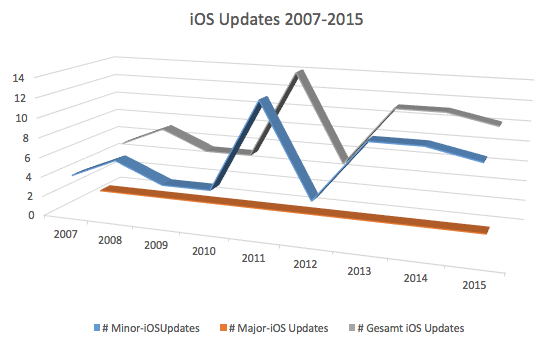
\includegraphics[scale=0.7]{Bilder/iOSUpdates}
        \caption{iOS Software Updates\cite{Apple[7]}}
        	\label{fig:iOS Software Updates}
\end{figure}

% ------ Hardcoded newpage -------
\newpage
Die „Jailbreak-Community“ benötigt im Durchschnitt 36 Tage, um eine neue iOS Version zu „jailbreaken“. Die „Bugs“, die ein Jailbreak ausnützt, sind meistens in mehreren iOS Versionen vorhanden. Nicht alle „Bugs“ werden von Apple geschlossen, es gibt Jailbreaks, die mehrere Jahre funktionieren. Dies gilt vor allem für ältere iOS Versionen und iOS Devices.

\begin{figure}[!ht]
        \centering
                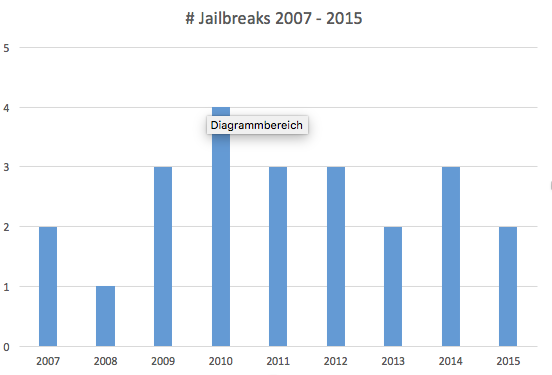
\includegraphics[scale=0.7]{Bilder/AnzahlJB}
        \caption{Anzahl iOS Jailbreak 2007 - 2015}
        	\label{fig:iOS Jailbreak}
\end{figure}


% ------------- Aufbau Jailbreak 9.x --------------------
\section{Aufbau Jailbreak iOS 9.x}
\label{sec:JBAufbau}
Damit ein Jailbreak auf einem iOS Device durchgeführt werden kann müssen Schritt für Schritt die iOS Sicherheitsschritte umgangen werden. Ab der iOS Version 8.1.3 sind für einen \glqq untethered Jailbreak\grqq{} fünf Schritte notwendig.

\begin{description}
\item[Dies sind die fünf iOS Sicherheitsmechanismen, die ein erfolgreicher Jailbreak umgehen muss]~\par
	\begin{enumerate}
	    \item Die Sandboxfunktionalität (siehe Kapitel: \ref{sec:Sandbox}) 
	     \item Das Signieren jedes Codes 
	    \item Erhalten der \glqq root\grqq{} Rechte
	    \item Das Patchen des Kernels
	  \end{enumerate}
\end{description} 

\cite{TaiG[1]}
\cite{TaiG[2]}
\cite{TaiG[3]}

% ------------- Jailbreak Step 1 --------------------
\subsection{Breaking out of the sandbox}
\label{sec:JBStep1}
Im ersten Schritt muss ein Bug im iOS und/oder einer Applikation gefunden werden, welcher es erlaubt \glqq die Sandbox\grqq{} (siehe Kapitel: \ref{sec:Sandbox}) zu umgehen. 

% ------------- Jailbreak Step 2 --------------------
\subsection{Obtaining arbitrary (unsigned) code execution}
\label{sec:JBStep2}

% ------------- Jailbreak Step 3 --------------------
\subsection{Obtaining root}
\label{sec:JBStep3}

% ------------- Jailbreak Step 4 --------------------
\subsection{Patching the Kernel}
\label{sec:JBStep4}
          % iOS Gundlagen
%----------------------------------------------------------------
%
%  File    :  chapter4.tex
%
%  Authors :  Michael Fuska, FH Campus Wien, Austria
% 
%  Created :  08 Feb 2016
% 
%  Changed :  
% 
%----------------------------------------------------------------
\chapter{Mobile Apple Betriebssystem iOS}
\label{ch:iOS}
%------------------------------------------------------------------------------
%---------------------------------- iOS Grundlagen
\section{iOS Grundlagen}
\label{sec:iOSGrundlage}

Das mobile Apple Betriebsystem iOS basiert auf dem Desktop Betriebssystem des Mac OS X. Darwin ist ein frei erhältliches Linux basiertes Betriebssystem.Dieses Betriebssystem stellt die Grundlage für das Mac OS X dar. Der Kernel des Mac OS X ist der XNU-Kernel mit entsprechenden Adaptionen für das Mac OS X und dem mobilen Betriebssystem iOS.
\begin{figure}[htbp]
        \centering
                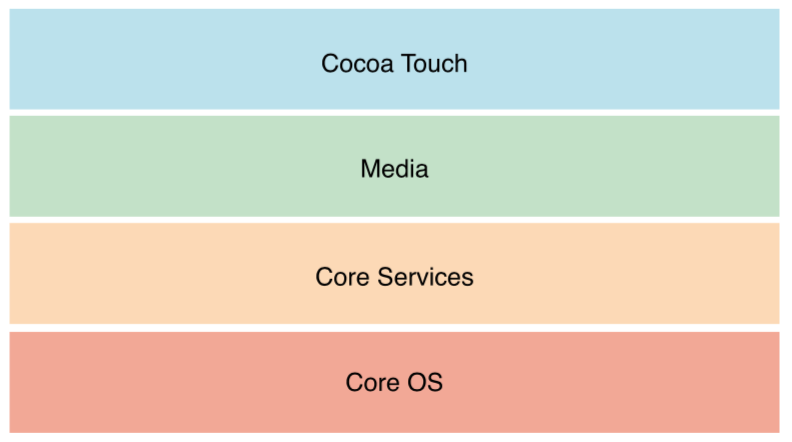
\includegraphics[height=5cm]{Bilder/Chapter3_SystemArchitektur}
        \caption{iOS Software Layer (\cite{Apple[6]}, S. XXXXXXXXX)}
        	\label{fig:iOS Software Layer}
\end{figure}
Die abgebildeten Schichten zeigen das abstrahiert iOS Betriebssystem. Der grösste Unterschied zwischen Mac OS X und iOS liegt im Cocoa Touch Layer.
  
\begin{description}
\item[Folgende \glqq Anforderungen\grqq{} werden an das iOS Software Layer Modell gestellt]~\par
	\begin{itemize}
		\item Sicherstellungen der \textbf{Datenintegrität}
		\item Gewährleistung der \textbf{Informationsvertraulichkeit}
		\item Sicherstellung der \textbf{User- und/oder Applikation Authentizität}
		\item Gewährleistung der \textbf{Daten/Informationsverbindlichkeit}
	\end{itemize}
\end{description}

%------------------------------------------------------------------------------
%---------------------------------- iOS Software Layer
\section{iOS Software Layer}
\label{sec:iOSSWLayer}

%---------------------------------- Core OS
\subsection{Core OS Layer}
\label{sec:CoreLayer}

Der \textbf{Core OS Layer} beinhaltet alle \textit{\glqq low-level Features\grqq{}} und auf diesen bauen alle anderen \textit{\glqq Frameworks\grqq{}} auf. iOS Applikationsentwickler kommen mit diesem Layer nur dann in Berührung, wenn sie sich mit der Sicherheit und mit Hardware-Kommunikation beschäftigen. 
\begin{description}
	\item[Core OS Layer Frameworks]~\par
	\begin{itemize}
		\item Accelerate Framework
		\item Core Bluetooth Framework
		\item External Accessory Framework
		\item Generic Security Service Framework
		\item Lost Authentication Framework
		\item Network Extension Framework
		\item Security Framework
		\item System
		\item 64-Bit Support
	\end{itemize}
\end{description}
 (vgl. \cite{Apple[6]}, S.49-52)
%---------------------------------- Core Service
\subsection{Core Service Layer}
\label{sec:CoreServiceLayer}		
Der \textbf{Core Service Layer} beinhaltet die fundamentalen System Services. Dieser Layer wird unterteilt in \textit{\glqq high-level Feature\grqq{}} und Core Services Frameworks.

\begin{description}
	\item[\textbf{High-level Feature dieses Layers}]~\par
	\begin{itemize}
		\item \textbf{Peer-to-Peer Services}
		\item \textbf{iCloud Storage}
		\item \textbf{Block Objects}
		\item \textbf{Data Protection}
		\item \textbf{File-Sharing Support}
		\item \textbf{Grand Central Dispatch}
		\item \textbf{In-App Purchase}
		\item \textbf{SQLite}
		\item \textbf{XML Support} 
	\end{itemize}
	
	\item[\textbf{Core Services Layer Frameworks}]~\par
	\begin{multicols}{2}
	\begin{itemize}
		\item Accounts Frameworks
		\item Address Book Framework
		\item Ad Support Framework
		\item CFNetwork Framework
		\item CloudKit Framework
		\item Core Data Framework
		\item Core Foundation Framework
		\item Core Location Framework
		\item Core Media Framework
		\item Core Motion Framework
		\item Core Telephony Framework
		\item EvenKit Framework
		\item Foundation Framework
		\item HealthKit Framework
		\item HomeKit Framework
		\item JavaScript Framework
		\item Mobile Core Services Framework
		\item Multipeer Connectivity Framework
		\item NewStandKit Framework
		\item PassKit Framework
		\item Quick Look Framework
		\item Safari Services Framework
		\item Social Framework
		\item StoreKit Framework
		\item System Configuration Framework
		\item WebKit Framework
	\end{itemize}
	\end{multicols}
\end{description}

(vgl. \cite{Apple[6]}, S.36-48)
%---------------------------------- Media Layer
\subsection{Media Layer}
\label{sec:MediaLayer}		
In diesem Layer sind alle Technologien zur Darstellung von Grafik, Video und das abspielen von Sound enthalten. Dieser Layer ist verantwortlich für das Design und den Sound der iOS Applikationen. 

\begin{description}
	\item[Dieser Layer stellt folgende Technologien zur Verfügung]~\par
    \begin{itemize}
		\item \textbf{Graphics Technologies}
		\item \textbf{Audio Technologies}
		\item \textbf{Video Technologies}
		\item \textbf{AirPlay}
    \end{itemize}

	\item[Media Layer Frameworks]~\par
	\begin{multicols}{2}
	\begin{itemize}
		\item Assets Library Framework
		\item AV Foundation Framework
		\item AVKit Framework
		\item CoreAudioKit Framework
		\item Core Graphics Framework
		\item Core Image Framework
		\item Core Text Framework
		\item Core Video Framework
		\item Game Controller Framework
		\item GLKit Framework
		\item Image I/O Framework
		\item Media Accessibility Framework
		\item Media Player Framework
		\item Metal Framework
		\item OpenGL ES Framework
		\item Photos Framework
		\item Photos UI Framework
		\item Quartz Core Framework
		\item SceneKit Framework
		\item SpriteKit Framework
         \end{itemize}
	\end{multicols}
\end{description}
(vgl. \cite{Apple[6]}, S.23-35)
%---------------------------------- Cocoa Touch Layer
\subsection{Cocoa Touch Layer}
\label{sec:CocoaTouchLayer}
Enthält die wichtigsten Frameworks um iOS Applikationen zu entwickeln. Dieser
Layer stellt die Basis Applikation Infrastruktur und folgende Key Technologien zur Verfügung

	\begin{itemize}
		\item \textbf{Multitasking}
		\item \textbf{Touch-based Input}
		\item \textbf{Push Notification}
		\item \textbf{High-level System Service}	
	\end{itemize}

\begin{description}
\item[Folgende Features sind in diesem Layer enthalten]~\par
	\begin{multicols}{2}
	\begin{itemize}
		\item App Extentision
		\item Handoff
		\item Document Picker
		\item AirDrop
		\item TextKit
		\item UIKit Dynamics
		\item Multitasking
		\item Auto Layout
		\item Storyboards
		\item UI State Preservation
		\item Apple Push Notification Service
		\item Local Notifications
		\item Gesture Recognizers
		\item Standard System View Controllers
         \end{itemize}
	\end{multicols}
	
	\item[Cocoa Touch Layer Frameworks]~\par
	\begin{multicols}{2}
	\begin{itemize}
		\item Address Book UI Framework
		\item EventKit UI Framework
		\item GameKit Framework
		\item iAd Framework
		\item MapKit Framework
		\item Message UI Framework
		\item Notification Center Framework
		\item PushKit Framework
		\item Twitter Framework
		\item UIKit Framework
         \end{itemize}
	\end{multicols}
\end{description}
(vgl. \cite{Apple[6]}, S.12-22)

%---------------------------------- iOS Device Security Architektur
\pagebreak
\section{iOS Device Security Architektur}
\label{sec:iOSSecArchitektur}

Der Sicherheitsmechanismus der iOS Device unterteilt sich in zwei Ebenen. 
\begin{figure}[htb]
  \begin{minipage}{0.6\textwidth} 
  		\begin{description}
   			\item[ iOS Sicherheitsebenen]~\par
         		\begin{enumerate}	
				\item  \textbf{iOS Software}
					\begin{enumerate}
       						\item File System
         					\item OS Partition
						\item User Partition (verschlüsselt)
						\item App Sandbox
						\item Data Protection Class
      					\end{enumerate}
      				\item  \textbf{iOS Hardware und Firmware}~\par
					\begin{enumerate}
       						\item Kernel
						\begin{enumerate}
						\item Secure Enclave
						\item Secure Element
         					\end{enumerate}	
						\item Crypto Engine
						\item Device Key
						\item Group Key
						\item Apple Root Certificate
      					\end{enumerate}
			\end{enumerate}
   		\end{description}
Die iOS Sicherheit passiert auf einer Kombination von Software, Hardware und Service um ein maximum an Sicherheit zu erreichen. (vgl. \cite{Apple[4]}, S.4)
	\end{minipage}
	\hfil
	\begin{minipage}{0.4\textwidth}
		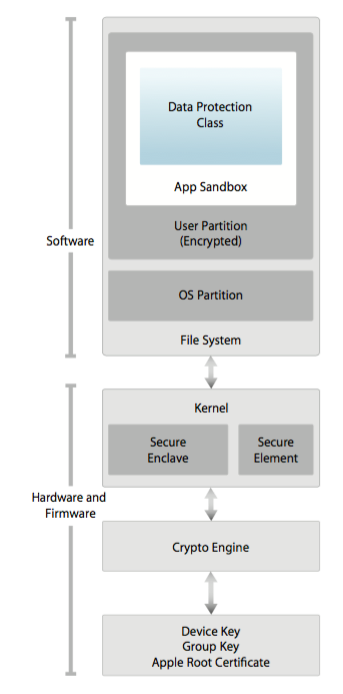
\includegraphics[width=\textwidth]{Bilder/Chapter3_SecArchitektur}
		\caption {iOS Security Architektur (\cite{Apple[4]}, S.4)}
        \label{fig:iOS Security Architektur}
	\end{minipage}
\end{figure}
		    	
%---------------------------- System Security
\subsection{System Security}
\label{sec:SystemSec}
Die \textbf{System Security} von iOS Device ist so kon­zep­ti­o­nie­rt, dass die Software und Hardware sicher über alle Kernkomponenten des Devices ist. Dies beinhaltet den sicheren Boot Prozess (Siehe Kapitel: \ref{sec:SecBootChain}), die Software Updates und die \textit{\glqq Secure Enclave \grqq{}} (Siehe Kapitel: \ref{sec:HardwareSecProtection}). Alle diese Maßnahmen dienen dazu, sicherzustellen, dass nur vertrauenswürdige Applikationen auf dem iOS Device ausgeführt werden können.\par 

Die enge Verbindung zwischen Hardware und Software eines iOS Geräte gewährleistet, dass alle Komponenten des Systems vertrauenswürdig sind, sowohl die Software als auch die Hardware. (vgl. \cite{Apple[4]}, S.5)
\begin{description}
\item[Apple führt unter dem Kapitel System Security folgende Features an]~\par
	%\begin{multicols}{2}
	\begin{itemize}
		\item Secure Boot Chain (siehe Kapitel:\ref{sec:SecBootChain})
 		\item System Software Authorization (siehe Kapitel:\ref{sec:SigningProcess})
 		\item Secure Enclave (Siehe Kapitel: \ref{sec:HardwareSecProtection})
 		\item Touch ID (Siehe Kapitel: \ref{sec:Passcode})
        \end{itemize}
	%\end{multicols}
\end{description}
(vgl. \cite{Apple[4]}, S.5-9)

%--------------------------- Encryption und Daten Sicherheit
\subsection{Encryption und Daten Sicherheit}
\label{sec:DataEnc}

Das iOS unterstützt standardmäßig eine Verschlüsselung und verschiedenste Datenschutzfunktionen für persönliche Daten und Unternehmensdaten. Die Sicherheitsinfrastruktur des iOS Devices ist so aufgebaut, dass selbst, wenn ein Teil des Betriebsystem kompromittiert ist, die anderen Bereiche des Devices, weiterhin sicher vor unerlaubten Zugriff sind. \par
Dies ist besonders für Unternehmen wichtig, da dadurch gewährleistet wird, dass vertrauliche Unternehmensdaten nicht gelesen werden können. Weitere iOS Features stellen sicher, dass selbst bei Diebstahl oder Verlust des iOS Devices die Daten sicher sind. Alle diese Features sind in der Standardkonfiguration aktiv gesetzt.


\begin{description}
\item[\parbox{\textwidth} {Apple führt unter dem Kapitel Encryption und Daten Sicherheit folgende Features an}]~\par
	\begin{itemize}
		\item \textbf{Hardware Security Features} (Siehe Kapitel: \ref{sec:HardwareSecProtection})
 		\item \textbf{File Data Protection} (Siehe Kapitel: \ref{sec:FileDataProtection})
 		\item \textbf{Passcodes} (Siehe Kapitel: \ref{sec:Passcode})
 		\item \textbf{Data Protection Classes}  (Siehe Kapitel: \ref{sec:HardwareSecProtection})
		\item \textbf{Keychain Data Protection} (Siehe Kapitel: \ref{sec:HardwareSecProtection})
	\end{itemize}
\end{description}
(vgl. \cite{Apple[4]}, S.10-17)

%------------------------------ Applikation Security
\subsection{Applikation Security}
\label{sec:AppSec}
Die Applikationen beinhalten das größte Sicherheitsrisiko für Betriebssysteme. Das Verhalten des Betriebssystems kann eine Applikationen negativ beeinflusst werden. Es kann die Sicherheit und die Verfügbarkeit des iOS Devices negativ beeinträchtigen. Des weiter kann die Integrität des Benutzerdaten durch unsicher Applikationen gefährdet werden.
\begin{description}
\item[\parbox{\textwidth} {Apple führt unter dem Kapitel Applikation Security folgende Features an}]~\par
	\begin{itemize}
		\item \textbf{App Code signing} (Siehe Kapitel: \ref{sec:SigningProcess}) 
		\item \textbf{Runtime process security} (Siehe Kapitel: \ref{sec:MemoryProtection})
		\item \textbf{Extensions}
		\item \textbf{App Groups} (Siehe Kapitel: \ref{sec:Sandbox})
		\item \textbf{Data Protection in Apps} (Siehe Kapitel: \ref{sec:SystemSec})

        \end{itemize}
\end{description}
(vgl. \cite{Apple[4]}, S.18-26)

%------------------------------ Network Security
\subsection{Network Security}
\label{sec:NetworkSec}
Die \textbf{ Netzwerk Sicherheit} ist ein wichtiger Bestandteil des Sicherheitskonzept und ergänzt die integrierten iOS Sicherheitsmechanismen. Die integrierten Sicherheitsmechanismen des mobilen Betriebssystem von Apple dienen dazu, die Daten auf dem Device zu schützen. Die Anforderungen an ein mobiles Device haben sich in den letzten Jahren dahin gehend verändert, dass der Zugriff auf externe Daten geschützt vorgenommen werden kann. Dieser Zugriff muss so abgesichert sein, dass die Datenübertragung sicher ist und die Usability des Produktes nicht eingeschränkt ist. Es werden Netzwerksicherheit Protokolle und Architekturen für eine authentifizierte, autorisierte und verschlüsselte Kommunikation verwendet.
\begin{description}
\item[\parbox{\textwidth} {Ein iOS Device verfügt über folgende Netzwerksicherheit Protokolle und Architekturen
an}]~\par
	\begin{itemize}
		\item \textbf{Virtual Private Network (VPN)}
 		\item \textbf{Single Sign-on}
 		\item \textbf{Internet Protocol Security (IPsec)}
 		\item \textbf{Transport Layer Security (TLS)} %(siehe Kapitel:\ref{sec:TLS})
		\item \textbf{Datagram Transport Layer Security (DTLS)}
        \end{itemize}
\end{description}
Des weiter werden die neuersten Standards für WLAN, Bluetooth und Mobilfunk-Verbindungen verwendet. (vgl. \cite{Apple[4]}, S.27-30)

%------------------------------ Apple Pay ----------------------------------
\subsection{Apple Pay}
\label{sec:ApplePay}

\textbf{Apple Pay} ist das interne Apple Zahlungssystem für mobile Geräte. Die Kommunikation findet über NFC statt. Neben NFC ist die App \textit{\glqq Wallet\grqq{}} Teil des Apple Pay Produkt.

\begin{description}
\item[\parbox{\textwidth} {Folgende Komponenten gehören zu dem Apple Pay Produkt}]~\par
	\begin{itemize}
		\item \textbf{Secure Element:} \\
        Alle Secure Element erfüllen den Industriestandard. Der zertifizierte Chip wird ein einer Java Card Plattform ausgeführt. Diese Elemente erfüllen den finanzindustrie Standard. 
 		\item \textbf{Near Field Communication (NFC) Controller:} \\
        Der NFC Controller und die NFC Kommunikation Protokolle sind für die Kommunikation zwischen den Anwendungsprozessoren und Secure Elementen zuständig.
 		\item \textbf{Wallet:} \\
        Die Wallet App ist für die Verwaltung der Kreditkarten und Debitkarten verantwortlich. 
            \begin{description}
                \item[\parbox{\textwidth} {Diese App ermöglicht es dem User}]~\par
                \begin{itemize}
                    \item die Kartendaten,
                    \item den Kartenaussteller,
                    \item die durchgeführten Transaktionen der einzelnen Karten und
                    \item vieles mehr
                \end{itemize}
            \end{description} 
        \textbf{abzuspeichern und anzuzeigen.}
        
 		\item \textbf{Secure Enclave:}\\
        Die Secure Enclave ist für den Authentifizierungsprozess einer Finanztransaktion zuständig. Des weiter werden in der Secure Enclave die Touch-ID Fingerabdrücke gespeichert.	
        \end{itemize}
\end{description}
(vgl. \cite{Apple[4]}, S.31-37)

%------------------------------ Internet services
\subsection{Internet Services}
\label{sec:InternetServices}

Apple hat sich die Prämisse gestellt stabile Applikationen mit guter Benutzbarkeit für den Benutzer zu entwickeln. 
\begin{description}
    \item[\parbox{\textwidth} {Beispiele für solche internen iOS Apps sind }]~\par
    \begin{itemize}
       \item iMessage,
       \item Facetime,
       \item iCloud und 
       \item iCloud Keychain.
    \end{itemize}
\end{description} 

Apple stellt den Entwicklern von Internet Diensten die Frameworks zur Verfügung, die auch für interne Apple Apps verwendet werden. Natürlich gelten für Internet Dienste die selben Sicherheitsziele, wie für die internen Apple Produkte. Diese Ziele beinhalten den \textit{\glqq sicheren Umgang mit den persönlichen Daten der Benutzer\grqq{}}, sowie \textit{\glqq den Schutz vor nicht autorisierten Zugriff auf die persönlichen Daten des Benutzers\grqq{}} und \textit{\glqq anderer Dienstleistungen\grqq{}}. Jeder Dienst verwendet eine eigene leistungsstarke Sicherheitsarchitektur ohne die Benutzerfreundlichkeit des gesamten iOS Devices zu beeinträchtigen. (vgl. \cite{Apple[4]}, S.38-49)

\begin{description}
    \item[\parbox{\textwidth} {Dies sind die Mainfeatures des Apple Internet Service}]~
    \begin{itemize}
        
        \item \textbf{Apple-ID:}\\
        Die \textbf{Apple-ID} ist Teil des persönliche Apple-Accounts, der zusammen mit dem \textit{\glqq Password\grqq{}} den Zugriff auf die Apple Service ermöglicht. 
        
        \item \textbf{iCloud:} \\
        Die \textbf{iCloud} ist der Apple Online-Dienst zum speichern und synchronisieren von Daten/Konfigurationen. 
        
        \item \textbf{iCloud Keychain:}\\
        Die \textbf{iCloud Keychain} ist das Apple Online \textit{\glqq Password Management System\grqq{}}. \begin{description}
                \item[\parbox{\textwidth} {Das Password Management System dient zum Speichern von}]~\par
                    \begin{itemize}
                        \item systemübergreifenden Passwörtern,
                        \item Login Daten,
                        \item WLAN-Zugangsdaten und 
                        \item Kreditkartendaten.
                    \end{itemize}
                \end{description} 
 
        \item \textbf{Continuity:}\\
        Darunter versteht Apple, dass Verteilen von Informationen und Services über mehrere iOS Devices. 
        \begin{description}
        \item[\parbox{\textwidth} {Beispiele für Continuity sind}]~\par
            \begin{itemize}
                \item Die Anrufannahme auf unterschiedlichen iOS Devices
                \item Die Möglichkeit Nachrichten auf unterschiedlichen iOS Devices zu lesen und zuschreiben.
                \item Das Verteilen von Dateien auf iOS Devices.
            \end{itemize}
        \end{description}  
    \end{itemize}
\end{description}

%------------------------------ Device Controls
\subsection{Device Controls}
\label{sec:DeviceControl}

Der \textbf{Device Control} Mechanismus von Apple hat die Aufgabe flexible Sicherheitsrichtlinien und Konfigurationen umzusetzen. Eine weitere Rahmenbedingung ist, dass die Konfiguration der Geräte leicht umsetzbar und verwaltbar ist.\par 
 Für Unternehmen bringt dies den Vorteil mit sich, dass Sicherheitsrichtlinien und Konfigurationen auf mehrere iOS Geräte verteilt werden können. Dadurch können Firmen sicherstellen, dass alle Geräte die selben Einstellungen besitzen. Des weiter ermöglicht es Mitarbeiter ihre eigenen Geräte im Unternehmen zu verwenden (BYOD). 

\begin{description}
    \item[\parbox{\textwidth} {Dies sind die Mainfeature des Apple Device Control Service} ]~\par
    \begin{multicols}{2}
    \begin{itemize}
        \item Passcode Sicherheit
        \item iOS pairing model
        \item Konfigurationsverteilung
        \item Mobile Device Management(MDM)
        \item Device Enrollment Program
        \item Device restriction
        \item Apple Configurator
        \item Supervised-only restrictions
        \item Remote wipe
        \item Find My iPhone and 
        \item Activation Lock
    \end{itemize}
    \end{multicols}
\end{description}
(vgl. \cite{Apple[4]}, S.50-55)
%----------------------------- Privacy Controls

\subsection{Datenschutzkontrolle}
\label{sec:PrivacyControls}
Das mobile Betriebssystem von Apple verfügt über zahlreiche integrierte Steuerelemente und Optionen. Diese iOS Einstellungen ermöglichen es dem Benutzer zu entscheiden, wie mit seinen persönlichen Daten umgegangen werden soll. Dies inkludiert welche App Zugriff auf welche Informationen bekommen soll. 

\begin{description}
    \item[\parbox{\textwidth} {Folgende Daten werden für die Ortung des Users verwendet (Location Service) }]~\par
    \begin{itemize}
        \item GPS Daten,
        \item Bluetooth Daten,
        \item öffentliche WLAN-Hotspots
        \item Mobilfunkmasten
    \end{itemize}
    Der User hat die Möglichkeit mit Hilfe von iOS Einstellungen zu definieren, welche App welche Location Daten verwenden kann.
    \item[\parbox{\textwidth} {Zu den persönlichen User-Daten zählen}]~\par
    \begin{multicols}{2}
    \begin{itemize}
        \item Kontakte
        \item Kalender
        \item Erinnerungen
        \item Fotos
        \item Aktivitätsdaten
        \item Accounts sozialer Netzwerke
        \item Mikrofon
        \item Kamera
        \item Bluetooth-Freigabe
    \end{itemize}
      \end{multicols}
\end{description}
(vgl. (\cite{Apple[4]}, S.56), (\cite{Apple[8]}, S.49))          % iOS Sicherheit Konzept

%
\appendix
% --- Verzeichnisse ------------------------------------------------------

\newpage
\chapter{Verzeichnisse}

% --- List of Figures ----------------------------------------------------

\newpage
\phantomsection
\addcontentsline{toc}{section}{Abbildungsverzeichnis}
\listoffigures



% --- List of Tables -----------------------------------------------------

\newpage
\phantomsection
\addcontentsline{toc}{section}{Tabellenverzeichnis}
\listoftables

% --- List of Listings -----------------------------------------------------

\newpage
\phantomsection
\addcontentsline{toc}{section}{Listings}
\lstlistoflistings

% --- Bibliography ------------------------------------------------------

\bibliographystyle{alpha}

% List references I definitely want in the bibliography,
% regardless of whether or not I cite them in the thesis.

\newpage
\phantomsection
\addcontentsline{toc}{section}{Literaturverzeichnis}
\bibliography{thesis}          % Appendix A

\end{document}

